

% A Readymade beamer presentation template
% Version 1.1
% Relase date: May 2, 2010
% Released at http://www.stattler.com
% by Rifat Jahan

\documentclass{beamer}
%\usecolortheme[named=green]{structure}
\mode<presentation> {
\usetheme{CambridgeUS}
\usecolortheme{orchid}
\usefonttheme{structuresmallcapsserif}
%\setbeamercovered{invisible}
% To remove the navigation symbols from the bottom of slides%
\setbeamertemplate{navigation symbols}{} 
}
 \setbeamertemplate{footline}
        {
      \leavevmode
      \hbox{
      \begin{beamercolorbox}[wd=.36\paperwidth,ht=2.25ex,dp=1ex,center]{author in head/foot}
        \usebeamerfont{author in head/foot}\insertshortauthor~~(\insertshortinstitute)
      \end{beamercolorbox}
      \begin{beamercolorbox}[wd=.56\paperwidth,ht=2.25ex,dp=1ex,center]{title in head/foot}
        \usebeamerfont{title in head/foot}\insertshorttitle
      \end{beamercolorbox}
      \begin{beamercolorbox}[wd=.08\paperwidth,ht=2.25ex,dp=1ex,right]{date in head/foot}
        \usebeamerfont{date in head/foot}\insertframenumber{}\hspace*{2em}

      \end{beamercolorbox}}
      \vskip0pt
    }

\usepackage{graphicx}
\title[Excepted Appointments and Presidential Unilateral Power]{Excepted Appointments and Presidential Unilateral Power}
%
\author{Emily Moore}
\institute[WUSTL]
{
Washington University-St. Louis \\
\medskip
{\emph{emily.moore@wustl.edu}}
}
\date{\today}
% \today will show current date. 
% Alternatively, you can specify a date.

\usepackage{Sweave}
\begin{document}
\Sconcordance{concordance:SPSA2016presentationslides.tex:SPSA2016presentationslides.Rnw:%
1 49 1 1 0 183 1}


%
\begin{frame}
\titlepage
\end{frame}
%
%

\begin{frame}
\frametitle{Presidents Influencing Policy}
\Large
\begin{itemize}\addtolength{\itemsep}{1\baselineskip}
\item Presidents have many tools for influencing legislative and administrative policymaking.
\item Appointment power is one of these tools (e.g., Moe 1985; Lewis 2008).
\item Excepted appointments are particularly useful but "invisible." (Lewis and Waterman 2013) 
\end{itemize}
\hfill%
\end{frame}


\begin{frame}
\frametitle{Elizabeth Warren and Antonio Weiss}
\begin{center}
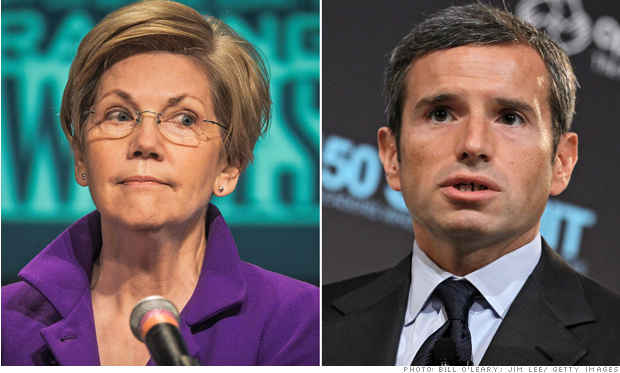
\includegraphics[height=2.6in,width=4in]{WarrenWeiss.png}

Elizabeth Warren and Antonio Weiss
\end{center}
\end{frame}

\begin{frame}
\frametitle{Lessons from the Warren/Weiss Story}
\Large
\begin{itemize}\addtolength{\itemsep}{1.5\baselineskip}
\item Two useful aspects of excepted appointments: flexibility and ideology
\item Excepted appointees can be used immediately.
\item They allow the president to appoint people Congress couldn't or wouldn't approve.
\end{itemize}
\hfill%
\end{frame}

%\begin{frame}
%\frametitle{Politics of Staffing the Bureaucracy}
%\Large
%\begin{itemize}\addtolength{\itemsep}{1.5\baselineskip}
%\item Presidents care about how agencies execute policy.
%\item Presidents face tradeoffs when making these decisions
%\item Presidents use both higher-level and lower-level appointees
%\item Ideology is an obvious consideration, but presidents have other considerations as well.
%\end{itemize}
%\hfill%
%\end{frame}

\begin{frame}
\frametitle{Ideology and Flexibility}
\begin{itemize}\addtolength{\itemsep}{1.5\baselineskip}
\item Traditional advice and consent takes an average of 265 days (Eilperin 2014) and 25 percent of appointees fail to make it through (O'Connell 2008).
\item The considerable cost and uncertainty surrounding the process discourages some excellent non-DC candidates (Eilperin 2014). 
\item Agencies differ in their propensity to follow directives and some are naturally more opposed to the president's agenda.
\item Presidents care about bringing opposing bureaus into line. Excepted appointments are one way to achieve this.
\end{itemize}
\hfill%
\end{frame}

\begin{frame}
\frametitle{Excepted Service and the Larger Appointment System}
\begin{columns}[T] % align columns
\begin{column}{.48\textwidth}
\begin{itemize}\addtolength{\itemsep}{1\baselineskip}
\item Excepted positions are all those excepted from the competitive service.
\item The excepted appointees referenced here are also exempt from advice and consent.
\item Eisenhower created Schedule Cs to help deal with bureaucratic expansion and cultivate trusted advisors. 
\item Schedule C appointees are created to serve in a "confidential or policy determining" position.
\end{itemize}
\end{column}%
\hfill%
\begin{column}{.48\textwidth}
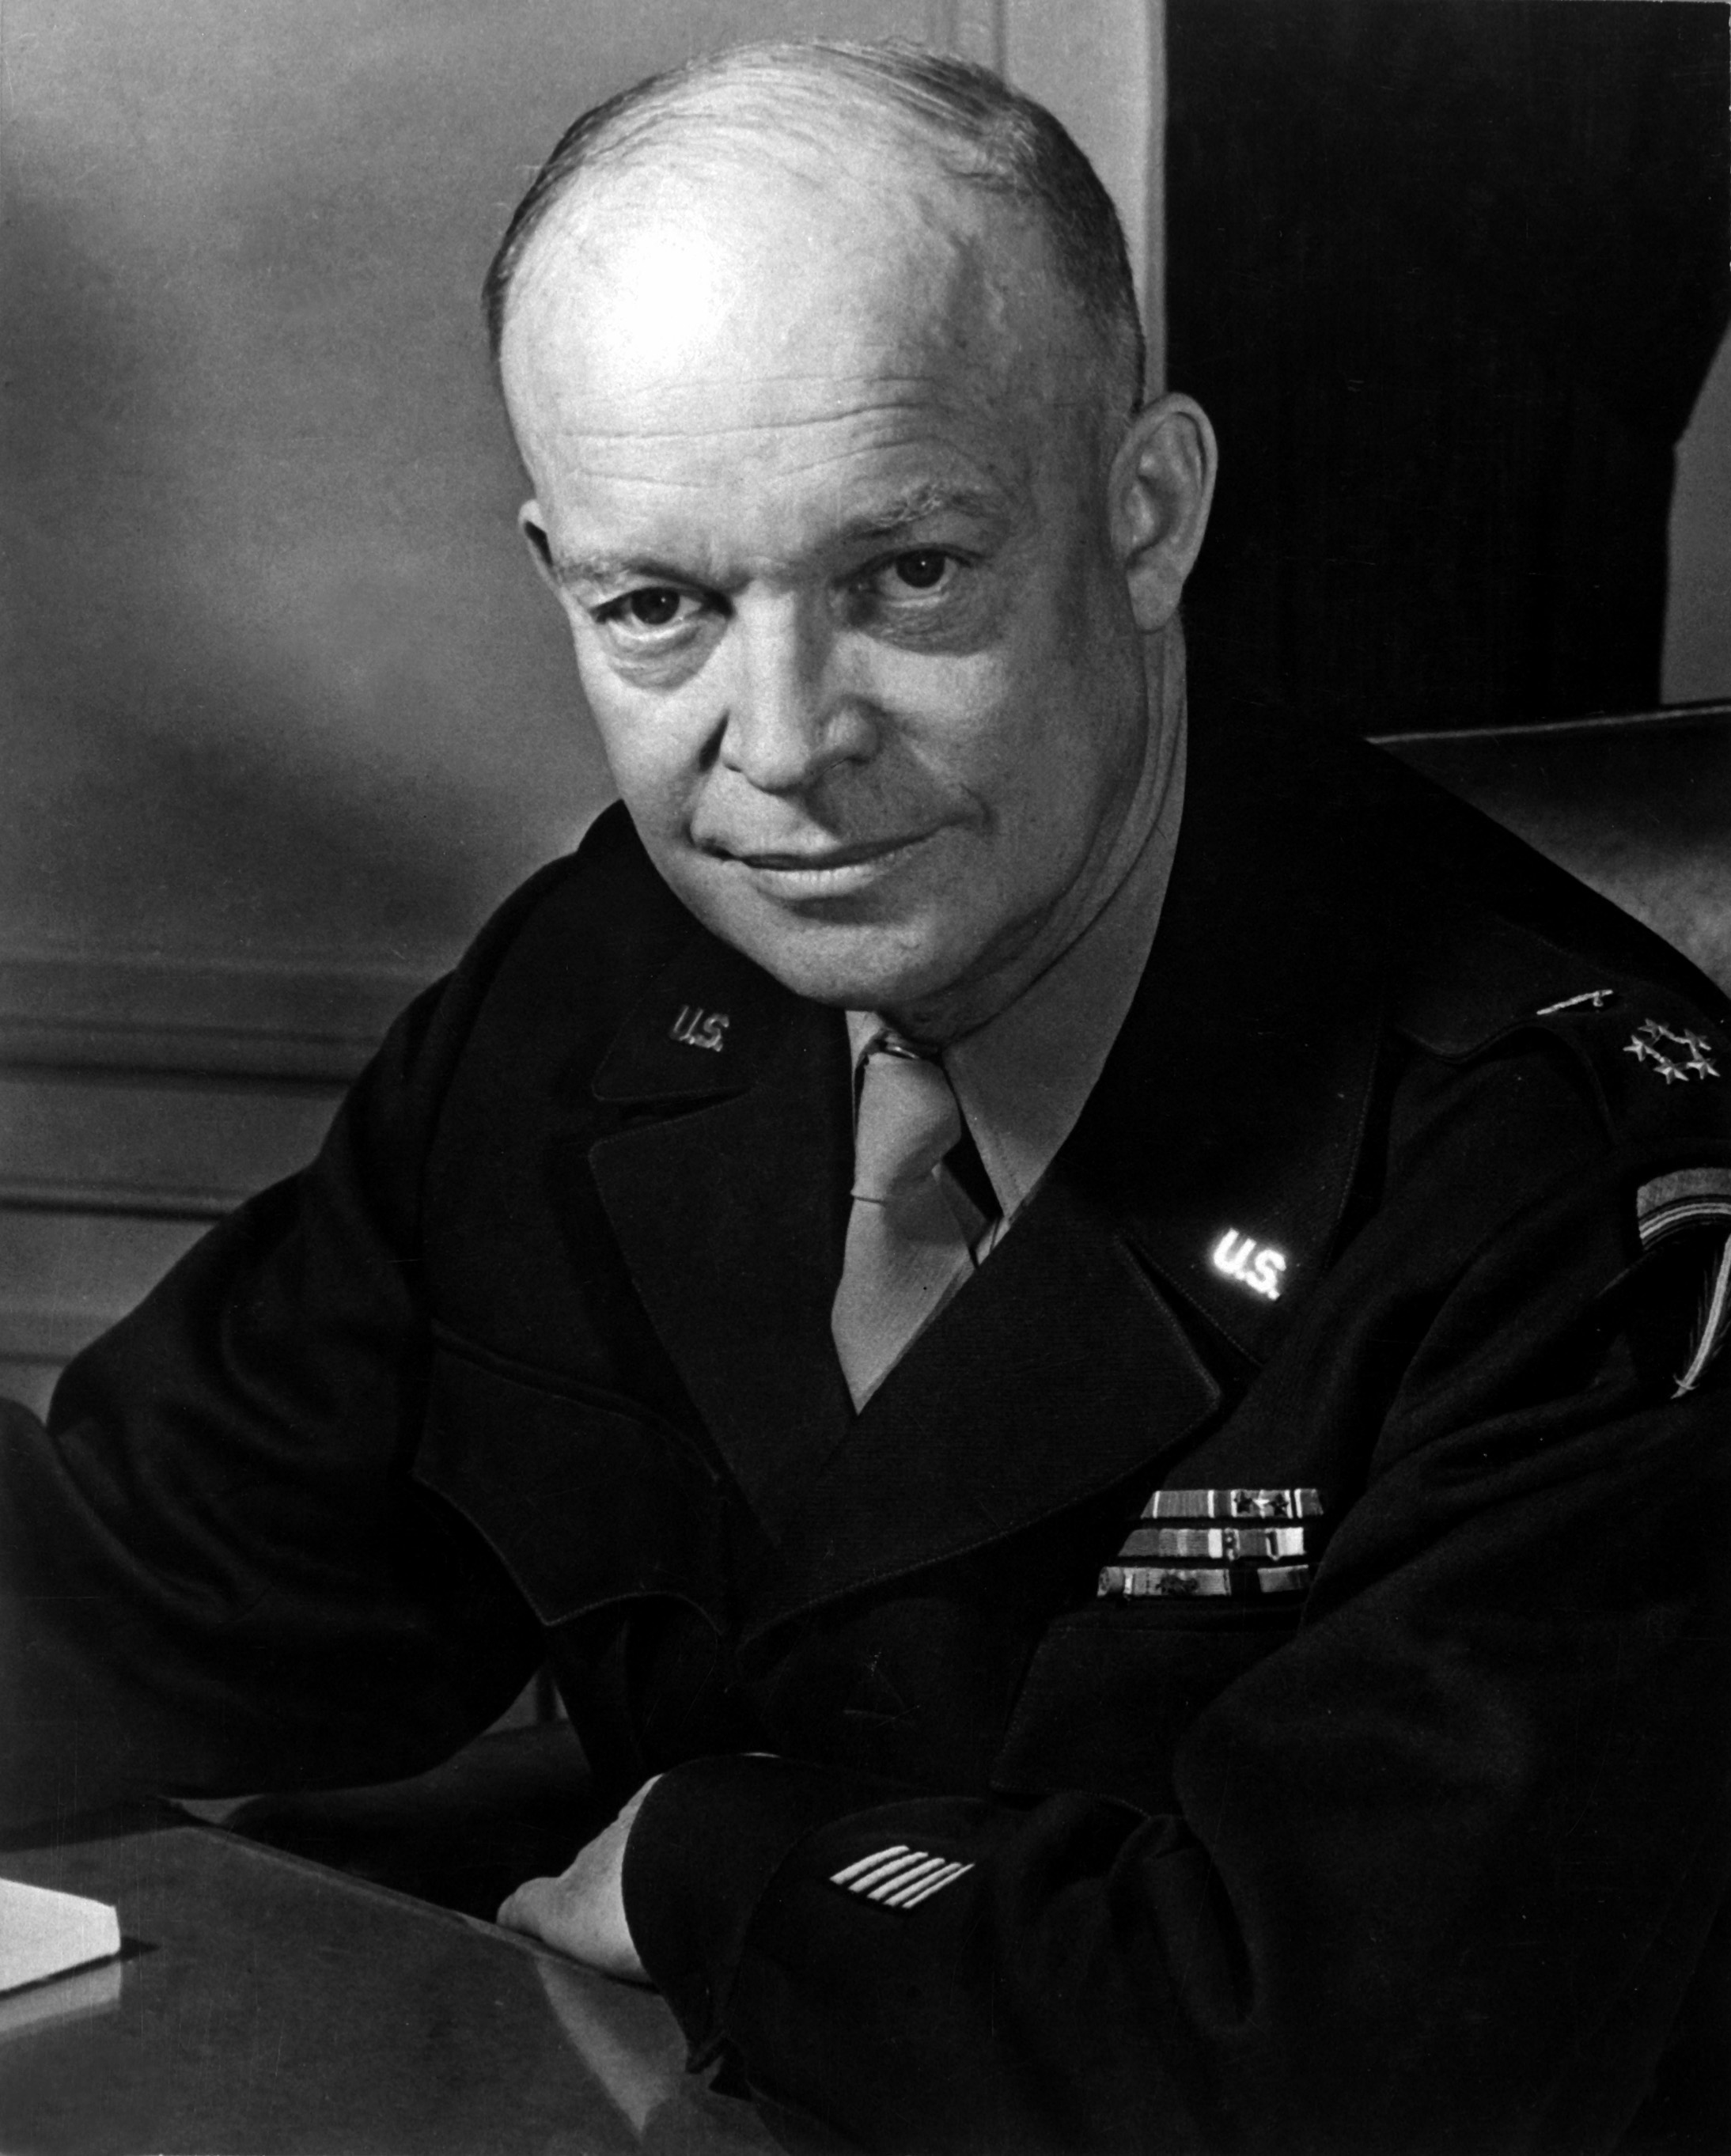
\includegraphics[height=2.5in,width=2in]{eisenhower.jpg}
\end{column}%
\end{columns}
\end{frame}

\begin{frame}
\frametitle{Examples of Schedule Cs in the larger system}
\begin{itemize}\addtolength{\itemsep}{1.5\baselineskip}
\item PAS appointees serve as department secretaries and undersecretaries as well as heads of independent agencies.
\item Deputy Undersecretaries are often non-career SES. 
\item Schedule Cs have many different jobs, but often serve as advisors on specific policy matters and sometimes approve the rulemaking activities of career staff or serve as liaison between political and career appointees.
\end{itemize}
\hfill%
\end{frame}

\begin{frame}
\begin{center}
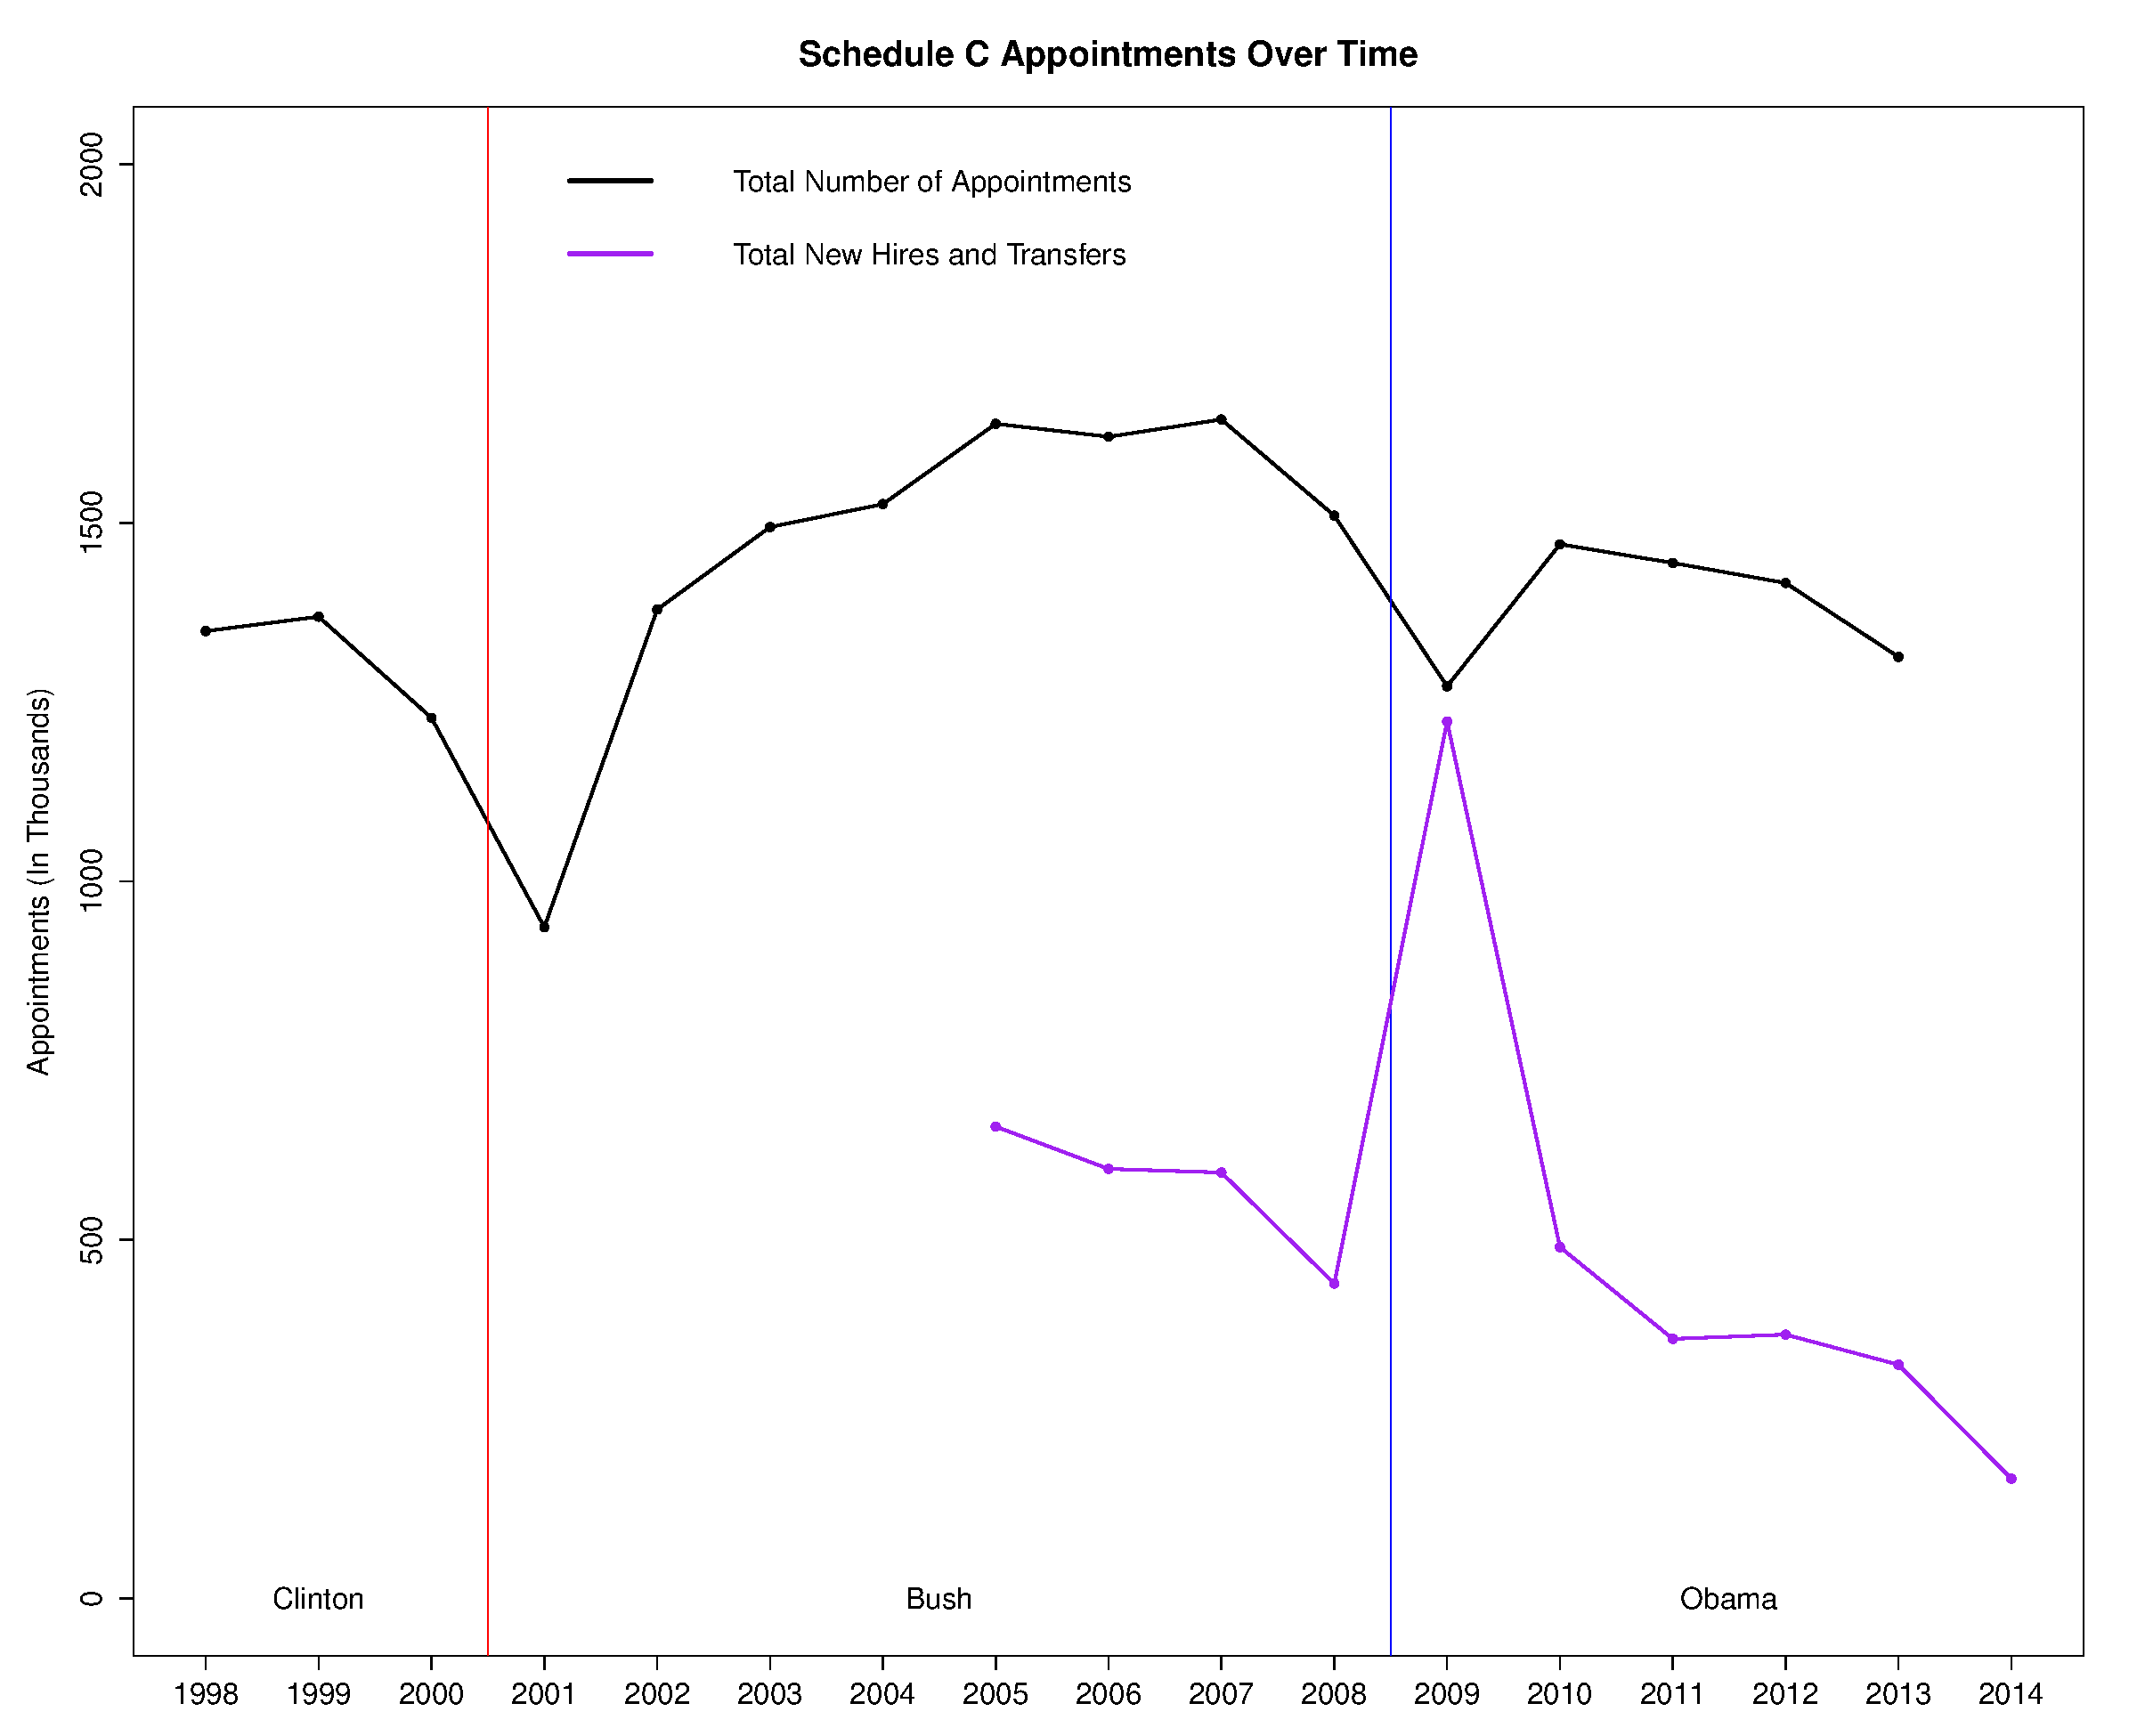
\includegraphics[height=3.5in,width=4.5in]{SCAptsandAccOverTime.pdf}
\end{center}
\end{frame}

\begin{frame}
\frametitle{Preliminary Evidence on Flexibility}
\begin{figure}[htb]
\begin{center}
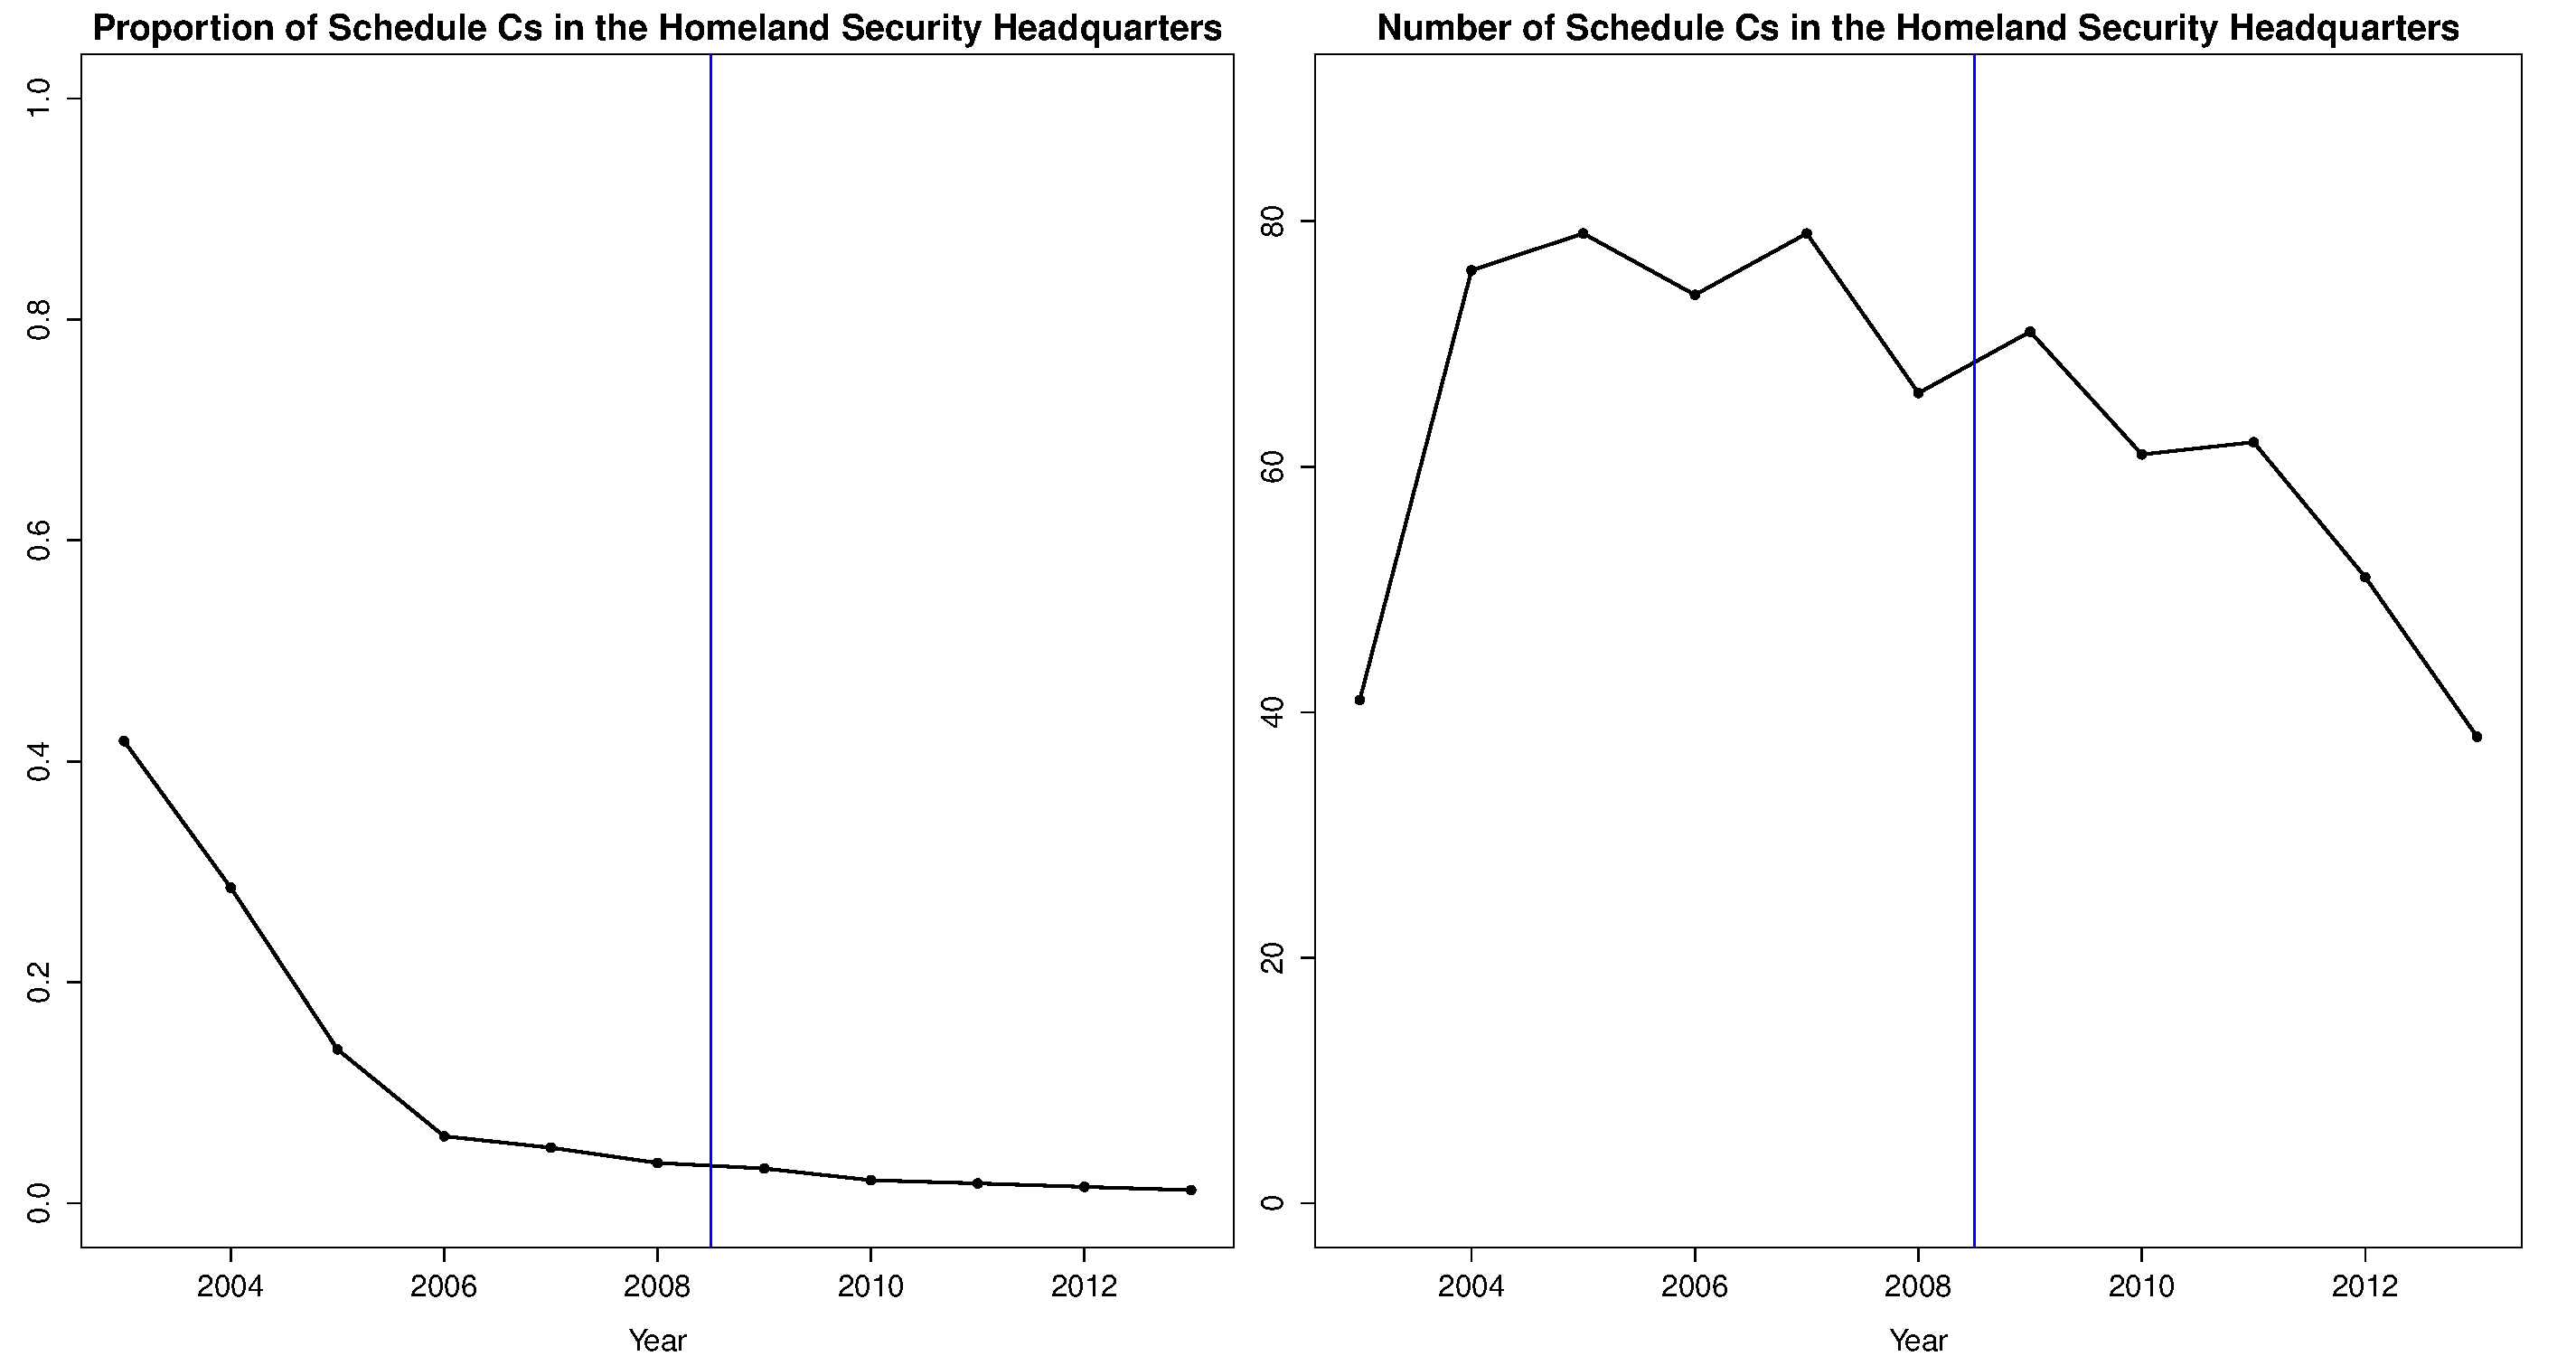
\includegraphics[height=2.75in,width=4.9in]{DHSProportionRawNumber.pdf}
\end{center}
\end{figure}
\end{frame}

\begin{frame}
\frametitle{Preliminary Evidence on Ideology}

\begin{itemize}\addtolength{\itemsep}{1.5\baselineskip}
\item The result is meant to serve as a validation of using Schedule C appointments to consider presidential unilateral power. 
\item Ideology is measured as the absolute distance between the agency ideal point and the president's ideal point.
\item Negative Binomial Regression Model.
\begin{itemize}\addtolength{\itemsep}{1\baselineskip}
\item Outcome Variable: Counts of Schedule C appointments in each agency 1998-2013.
\item Model includes ideology measure, presidential dummies, a unified government indicator, and agency fixed effects.
\end{itemize}
\end{itemize}
\end{frame}

\begin{frame}[fragile]
\frametitle{Ideology Results}
\tiny
\begin{table}[!h] \centering 
  \caption{Negative Binomial Regression Models of Appointments and Ideology} 
  \label{} 
\begin{tabular}{@{\extracolsep{5pt}}lcc} 
\\[-1.8ex]\hline 
\hline \\[-1.8ex] 
 & \multicolumn{2}{c}{\textit{Dependent variable: Count of Schedule C Appointees}} \\ 
\cline{2-3} 
\\[-1.8ex] & \multicolumn{2}{c}{} \\ 
\\[-1.8ex] & Model 1 & Model 2\\ 
\hline \\[-1.8ex] 
 Ideology & 0.056 & 0.307 \\ 
  & (0.029) & (0.081) \\ 
  & & \\ 
 Clinton & $-$0.086 & $-$0.190 \\ 
  & (0.034) & (0.170) \\ 
  & & \\ 
 Obama & $-$0.086 & $-$0.119 \\ 
  & (0.026) & (0.126) \\ 
  & & \\ 
 Unified Government & $-$0.051 & $-$0.061 \\ 
  & (0.025) & (0.126) \\ 
  & & \\ 
 Constant & 3.267 & 2.735 \\ 
  & (0.074) & (0.137) \\ 
  & & \\ 
  Fixed Effects & yes & no\\
\hline \\[-1.8ex] 
Observations & 1,213 & 1,213 \\ 
Log Likelihood & $-$2,523.319 & $-$4,248.940 \\ 
$\theta$ & 38.152  (5.129) & 0.311  (0.013) \\ 
Akaike Inf. Crit. & 5,210.637 & 8,507.880 \\ 
\hline 
\hline \\[-1.8ex] 
\end{tabular}
\end{table} 
\end{frame}

\begin{frame}[fragile]
\frametitle{Conclusion}
\begin{itemize}\addtolength{\itemsep}{1\baselineskip}
\item Excepted appointments allow the president the flexibility he needs to make many appointments quickly.
\item The case of the Department of Homeland Security headquarters suggests these appointees can be used to fill positions quickly in a brand new and very salient agency.
\item A preliminary regression model also suggests that the president places Schedule C appointees into ideologically dissimilar agencies, perhaps to bring naturally opposed bureaus more in line with his policy agenda.
\item Overall, this project is meant to serve as evidence that Schedule C appointees are a tool in the president's unilateral toolbox and deserve further study.
\end{itemize}
\end{frame}


\end{document}









